\documentclass[11pt]{article}


\usepackage{epsfig}
\usepackage{graphicx}
\usepackage{latexsym}
\usepackage{amsmath}
\usepackage{amssymb}
\usepackage{tikz}
\usetikzlibrary{arrows}
\usepackage{setspace}
\doublespacing

\setlength{\textwidth}{6.0in}
\setlength{\oddsidemargin}{.1in}
\setlength{\textheight}{21.5cm}
\setlength{\topmargin}{-1.cm}

\setlength{\parindent}{2 ex}
\def\noi{\noindent}
\def\sma{\smallskip}
\def\med{\medskip}
\def\big{\bigskip}

\newtheorem{theorem}{Theorem}
\newtheorem{proposition}{Proposition}
\newtheorem{lemma}{Lemma}
\newtheorem{corollary}{Corollary}
\newtheorem{conjecture}{Conjecture}
\newtheorem{definition}{Definition}
\newtheorem{claim}[theorem]{Claim}
\newtheorem{lem}[theorem]{Lemma}
\newtheorem{prob}{Problem}
\newcommand{\cqfd}{\mbox{}\hfill $\Box$ \medskip}
\newcommand{\comment}[1]{}

\title{De Novo Assembly of Distance Maps using on the fly Multiple Alignment Consensus Construction}
%Map Assembly of Tagged, Hybridized Sequences \newline(MATHS)}
%Positional Assembly of Nanopore Translocated Sequences (PANTS)}
\date{10 Sept 2012} %Clears date field from title
\author{Peter Goldstein, William Heaton}
\begin{document}
\maketitle

\paragraph{Background and Definitions\newline}
\par{
We define a \textbf{genetic map} (hereafter \textbf{map}) to be a set of ordered distance between \textbf{events} on a biopolymer, including but not limited to DNA. Such a map may have annotations on the events themselves indicating additional information, such as the identity of the biopolymer sequence at this location (hereafter \textbf{tags}). This data can be acquired in several ways.  Initially biologists measured linkage disequilibrium between different phenotypic or genotypic variants by breeding many individuals of a species and determined a physical distance between sites based on the level of recombination between those sites as measured by the resulting phenotypes.  Other distance maps in genetics are ordered restriction digestion maps.  These may be constructed algorithmically from multiple co-restriction digestions along with measuring the size of the resultant fragments via gel electrophoresis. Or they may be acquired via direct optical detection of DNA fixed on a surface, labeled with fluorophores, and restriction digested enzymatically as they are in the so called \textbf{Optical Mapping} system that the company Opgen has pioneered \cite{Opgen0}\cite{Opgen2}\cite{Opgen3}. A newer example of a genetic map technology is  an electronic DNA map generated by \textbf{Nabsys Positional Sequencing} technology.  In this technology, DNA bound with \textbf{sequence-specific probe molecules} is translocated through a nanopore from which the blockade of electrical current is used to detect the DNA and its probes.  

}
\par{
A single map may have sites corresponding to multiple different sequences.  This heterogeneity could result from using a mixture of probe molecules, using a single probe molecule that targets multiple sequences, a combination of these two, or other approaches.  In the case where a single map is produced using a mixture of probe molecules, these probes might have a sufficiently different chemical makeup as to produce differentiable signal traces in the Nabsys instrument.  In this case, the genetic map would consist of a set of ordered distances (\textbf{intervals}) between probe binding events (\textbf{probe sites}) as well as an annotation as to the probable identity of identities of each probe site (\textbf{tags}).
 }
 
 
\paragraph{Motivation\newline}
\par{
This type of information can be thought of as a relatively low resolution measurement of DNA sequence where the highest possible resolution would be the entire DNA sequence.  But since several technologies available are able to create genetic maps in a fraction of the amount of time and money that full sequencing can be done for it is often advantageous to work with such data.  Also with current sequencing technologies, long range information is not available and therefore the final sequence data is segmented into small contiguous sequences.  This is due mostly to repeat regions in the genome longer than the read lengths that current high throughput sequencing technologies can attain.  These repeat regions create ambiguities in how to put together the reads and therefore create discontinuities in the resulting assembly.  The technologies that create distance maps do not have this shortcoming as their ``reads" are far longer than the longest repeated sequence in the genome.  These maps are useful as supplementary data as a source of orthogonal information which can be combined with sequencing data for a more complete and correct measurement of the genome\cite{AMOS}\cite{OpgenMaize}\cite{OpgenHuman}.  It is also possible to obtain the full sequence data via many mapping experiments with a library of sequence specific probes and combining that data into single base resolution sequence data.


}


\paragraph{Goals\newline}
\par{
There are several common goals in dealing with genetic maps.  The main goal is to determine the true underlying distance map for whatever feature (most commonly sequence specific) you are targeting over the entire genome.  This is complicated by the fact that no technology can isolate and measure DNA molecules of the length of chromosomes.  

Because of this, the so-called shotgun method is used.  This method entails fragmenting several copies of the genome randomly and making measurements of these fragments.  Because there were multiple copies of the genome to start with and the fragmentation is a random process, some \textbf{fragments} will be \textbf{overlapping} measurements of the same locus in the genome. Then by comparing measurements that overlap on one region of the genome but extend in either direction these can be combined to grow the contiguous multi-measurement further.  This process is repeated until hopefully each chromosome is contained in a single contiguous multi-measurement. From this multi-measurement errors in individual measurements are reduced or eliminated based on averaging and voting over many measurements to produce a very reliable consensus map.  
%This last step is made possible with a \textbf{multiple alignment} which we will define further later in this document.
}


\par{
First we concern ourselves with identifying homology between genetic maps.  A pair of maps might share homology for a number of reasons.  First, a pair of maps might be approximate measurements of the same biopolymer, two biopolymers that are identical copies of a source molecule, or two biopolymers that are copies (identical or approximate) of overlapping regions of a source molecule.  In this last case, we say that these two measurements (\textbf{fragments}) \textbf{overlap}. 

%Second, a pair of genetic maps might originate from biopolymers from ancestrally related organisms. 
%In this case, expected homology refers to the most recent shared ancestor between the two organisms in question. In either of these cases, a pair of maps that share homology is assumed to share a "common origin" and to result from applying a process of modifications on this origin map.  

In the case of approximate measurements with error, the error process is assumed to be a source of random noise described by probability distributions.  Nabsys electronic maps have noise resulting from the random thermodynamic process of annealing probes to target, variable molecular configuration (including velocity and brownian motion) during molecular sensing, and variation in electronic signal.  These sources of noise result in uncertainty in interval sizing (\textbf{positional error}), missing probe sites (\textbf{false negatives}), erroneous probe site detections (\textbf{false positives}), and uncertainty in probe site identity (\textbf{tag call probabilities}).  

%In the case of ancestrally related maps, the process of modification is much more diverse, but can include local replacements in the biopolymer, translocation of a segment of the biopolymer to a different location or orientation, and duplication of a segment at a neighboring or different location.  

Here we are primarily concerned with the case of overlapping fragments as previously defined.  In the following sections we will briefly describe comparisons (in particular a type of comparison called an \textbf{alignment}) of pairs of maps to determine if they share a homologous overlapping region and if so exactly how they overlap.  Then we will describe a novel method for comparing multiple ($>2$) overlapping maps at once.  And finally we will describe a novel De novo assembly strategy using these tools.  

%Furthermore we will describe novel methods for using these assembled genetic maps in concert with short read sequencing data such as that produced by Illumina sequencers to provide a more accurate and complete measurement of the genome.
}


%\par{
%In addition to error correction, multiple alignment assists in joining together neighboring fragments.  Suppose that a physical process has caused the input DNA sample to sheer at random. Suppose also that the DNA sample consisted of several copies of the same genome.  Measurements of these DNA fragments, therefore, give overlapping measurements at each point on the genome.  But since the different copies of the genome are presumed to have broken at different, uncorrelated locations, overlapping DNA fragments will, with high probability, bridge the break points between neighboring fragments.  Thus whereas the set of measurements overlapping a particular zone in the genome can only provide a multiple alignment describing their overlap region, bridging fragments across neighboring zones can recover the adjacency of these zones, building a more complete map than the raw measurements themselves provide.  This process of coming up with a contiguous consensus map from many overlapping measurements is referred to as \textbf{assembly}.
%}


\paragraph{Pairwise Map Alignment\newline}
\par{
Thanks to Waterman and others, there exists a considerable literature on pairwise map alignments.\cite{Waterman84}\cite{Waterman1}\cite{ValouevAlignment}\cite{SOMA}  They are similar to algorithms for pairwise sequence alignment originally by Needleman and Wunsch\cite{NeedlemanWunsch} and extended by Smith and Waterman.\cite{SmithWaterman}\cite{Durbin}  These algorithms construct an ordered set of matched pairs of events between the two input maps such that a score function on the level of error admitted by the alignment is optimized (maximized or minimized depending on scoring metric over all possible alignments).  Since this is all previous work not novel to our method we will simply refer the reader to appropriate sources and provide one example.  In the example below the horizontal lines represents the two DNA fragments and the tick marks represent events.  Here you can see the distance between each tick represents the distance between each event.  Further, the dotted lines between ticks on the other strand represent the alignment of those probes.  The ordered set of pairs of probes aligned in the optimal alignment are the pairwise alignment between two fragments.  For notation we will denote $v^{i}_j$ as the $j^{th}$ event on map $i$. }

%Pairwise Alignment
\begin{figure}[h!]
 \caption{Pairwise Map Alignment.}
\begin{center}
\begin{tikzpicture}[scale=1]

	\tikzstyle alignment lines=[densely dashed, thick];
	\tikzstyle fragment lines=[thick];
	\tikzstyle probe lines=[thick];

	\draw[fragment lines] (-6,1) node[anchor=east] {$v^0$} -- (3.5,1);
		\foreach \x/\label in {-5.8/0,-5.5/1,-2.75/2,-2.5/3,0/4,2/5,3/6}
			\draw[probe lines,xshift=\x cm] (0,.85) -- (0,1.15) node[anchor=south] {$\label$};

	\draw[fragment lines] (-3.5,0) node[anchor=east] {$v^1$}  -- (6,0);
		\foreach \x/\y in {-2.75/0,-2.5/1,0/2,2/3,3/4,4.5/5,5/6}
			\draw[probe lines,xshift=\x cm] (0,.15) -- (0,-.15) node[anchor=north] {$\y$};
		
		\foreach \x in {-2.75,-2.5,0,2,3}
			\draw[alignment lines, xshift=\x cm] (0,.18) -- (0,.82);

\end{tikzpicture}

\end{center}
\end{figure}
\begin{center}
Giving the ordered set of pairs for this alignment as $\{\{v^0_2,v^1_0\},\{v^0_3,v^1_1\},\{v^0_4,v^1_2\},\{v^0_5,v^1_3\},\{v^0_6,v^1_4\}\}$
\end{center}

 If the score of such an alignment meets certain statistical tests the maps are homologous.  In the case of shotgun assembly, when an alignment score passes these tests the two fragments most likely arose from copies of overlapping regions of the source molecule.  Also, the aligned pairs of events in such an alignment are likely to represent measurements of the same particular locus in the genome.

\par{
Later in this document it will become useful to diagram this alignment as a graph where the events are vertices and an edge represents the fact that those two events have been aligned.  This seems rather trivial for the pairwise case but will become more complex later.  An example of this can be seen in Figure 2.
}
\begin{figure}[h!]
\begin{center}
\begin{tikzpicture}[scale=1]

	\tikzstyle probe=[thick];
	\tikzstyle fragment lines=[thick];
	\tikzstyle probe lines=[thick];

	\foreach \x/\label in {-5.8/0,-5.5/1,-2.75/2,-2.5/3,0/4,2/5,3/6}
			\filldraw[probe,xshift=\label cm] (0,1) circle (1.75pt) node[anchor=south] {$v^0_\label$};
			
			\foreach \x/\label in {2/0,3/1,4/2,5/3,6/4,7/5,8/6}
			\filldraw[probe,xshift=\x cm] (0,0) circle (1.75pt) node[anchor=north] {$v^1_\label$};
			
			\foreach \x in {2,3,4,5,6}
				\draw[probe lines,xshift=\x cm] (0,0) -- (0,1);


	%\filldraw[probe] (-6,0) circle (1.75pt);
		
	

\end{tikzpicture}
\caption{Pairwise Map Alignment: Graph Representation. Note that the distances between events is not encoded in this representation.  Because the alignment was based on that information all we care about here is that resultant alignment.}

\end{center}
\end{figure}


\paragraph{Pairwise Alignment Errors\newline}
\par{
While representing the optimal scoring alignment, a pairwise alignment can have errors.  Generally speaking, then, we can define two kinds of errors in a pairwise alignment: missing edges and extra edges.  That is to say two events that should have been aligned as they represent measurements of the same location in the genome but were not aligned and two events that should not have been aligned because they represent two different locations in the genome but were aligned.  It is important to note that this second case may occur either because the fragments themselves arose from different locations in the genome or when a local error of aligning two events that because of positional error or false positives and false negatives appeared to be the same event under the tolerated error.  The diagrams below demonstrate some causes of alignment errors.  Note that false positive measurements are colored red here.  And the false negatives are shown by an outline shaded red in the place where the event should have occurred.  In real data of course we do not know which probes are false positives and if or where an event should have occurred so we are displaying this information for demonstration purposes only. The error in the data must be modeled and incorporated in a scoring system that minimizes these alignment errors \cite{Sarkar}\cite{Nguyen}
}

\begin{figure}[h!]

\begin{center}
\begin{tikzpicture}[scale=1]

	\tikzstyle alignment lines=[densely dashed, thick];
	\tikzstyle fragment lines=[thick];
	\tikzstyle probe lines=[thick];
	\tikzstyle false positive=[color=red,thick];

	\draw[fragment lines] (-6,1) node[anchor=east] {$v^0$} -- (3.5,1);
		\foreach \x/\label in {-5.8/0,-5.5/1,-2.75/2,-2.5/3,0/4,2.2/6,3/7}
			\draw[probe lines,xshift=\x cm] (0,.85) -- (0,1.15) node[anchor=south] {$\label$};
			
			\draw[false positive] (.2,.85) -- (.2,1.15) node[anchor = south] {5};

	\draw[fragment lines] (-3.5,0) node[anchor=east] {$v^1$}  -- (6,0);
		\foreach \x/\y in {-2.75/0,-2.5/1,0/2,2/3,3/4,4.5/5,5/6}
			\draw[probe lines,xshift=\x cm] (0,.15) -- (0,-.15) node[anchor=north] {$\y$};
		
		\foreach \x in {-2.75,-2.5,3}
			\draw[alignment lines, xshift=\x cm] (0,.18) -- (0,.82);
			
			\draw[alignment lines] (2,.18) -- (2.2,.82);
			\draw[alignment lines] (0,.18) -- (.2,.82);

\end{tikzpicture}
 \caption{Alignment errors.  As you can see here, positional error along with a false positive have created an alignment error.  There is a missing alignment between $v^0_4$ and $v^1_2$ as well as an erroneous edge between $v^0_5$ and $v^1_2$.}
\end{center}
\end{figure}

\begin{figure}[h!]

\begin{center}
\begin{tikzpicture}[scale=1]

	\tikzstyle alignment lines=[densely dashed, thick];
	\tikzstyle fragment lines=[thick];
	\tikzstyle probe lines=[thick];
	
	\filldraw[red!30, thick] (-2.8,-.2) rectangle +(.115,.4);
	\draw[thick, densely dotted] (-2.8,-.2) rectangle +(.115,.4);

	\draw[fragment lines] (-6,1) node[anchor=east] {$v^0$} -- (3.5,1);
		\foreach \x/\label in {-5.8/0,-5.5/1,-2.75/2,-2.5/3,-0.2/4,2/5,3/6}
			\draw[probe lines,xshift=\x cm] (0,.85) -- (0,1.15) node[anchor=south] {$\label$};

	\draw[fragment lines] (-3.5,0) node[anchor=east] {$v^1$}  -- (6,0);
		\foreach \x/\y in {-2.5/0,0/1,2/2,3/3,4.5/4,5/5}
			\draw[probe lines,xshift=\x cm] (0,.15) -- (0,-.15) node[anchor=north] {$\y$};
		
		\foreach \x in {2,3}
			\draw[alignment lines, xshift=\x cm] (0,.18) -- (0,.82);
			
			\draw[alignment lines] (0,.18) -- (-.2,.82);
			\draw[alignment lines] (-2.5,.18) -- (-2.75,.82);

		

\end{tikzpicture}
 \caption{Alignment errors.  Here we have the contrapositive to the previous example in which positional error and a false negative combine to create an alignment error.  We will not show it but it is easy to imagine positional error alone creating a miss alignment (the simplest example would be that two events that should have been aligned were not because their positions were simply too distantly perturbed.  The "decision" to call 2 false positives instead of aligning two poorly distance matching events depends on the scoring metric which should be based on the relative error models of false positives/false negatives and positional error.}
\end{center}
\end{figure}

\paragraph{\newline Multiple Alignment\newline}


\par{
We shall describe the homology between a set of \textbf{input maps} with a multiple alignment.  The purpose of a multiple alignment is to match input map events in sets that reflect the target feature occurrences on the source molecule from which the inputs originated.  In structure, a multiple alignment is an ordered set of sets of probe sites. Each set (\textbf{aligned point}) consists of at most one probe landing on each measurement map.  Additionally, each probe landing on each measurement map is present in at most one set. Finally, the sets must obey the ordering principle: if events a, b, and c occur on the same input map such that b lies after a and before c, and each of a, b, and c is in an aligned point, the the aligned point containing b lies after the aligned point which contains a and before that which contains c in the multiple alignment.  Intuitively, each aligned point consists of those events that "match," i.e. that are measurements of the same locus in the genome.
}

\begin{figure}[h!]

\begin{center}
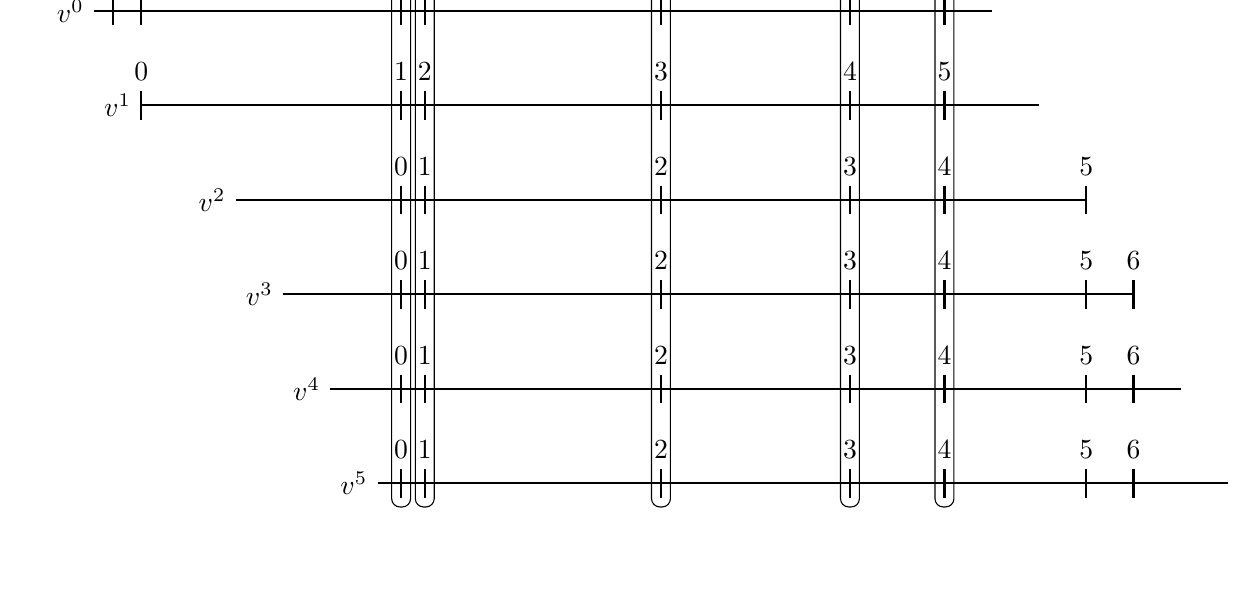
\begin{tikzpicture}[scale=1.2]

	\tikzstyle alignment lines=[densely dashed, thick];
	\tikzstyle fragment lines=[thick];
	\tikzstyle probe lines=[thick];
	\tikzstyle multiple alignment=[rounded corners=3pt];

	\draw[fragment lines] (-6,5) node[anchor=east] {$v^0$} -- (3.5,5);
		\foreach \x/\label in {-5.8/0,-5.5/1,-2.75/2,-2.5/3,0/4,2/5,3/6}
			\draw[probe lines,xshift=\x cm] (0,4.85) -- (0,5.15) node[anchor=south] {$\label$};

	\draw[fragment lines] (-5.5,4) node[anchor=east] {$v^1$}  -- (4,4);
		\foreach \x/\y in {-5.5/0,-2.75/1,-2.5/2,0/3,2/4,3/5}
			\draw[probe lines,xshift=\x cm] (0,4.15) node[anchor=south] {$\y$} -- (0,3.85) ;
			
			\draw[fragment lines] (-4.5,3) node[anchor=east] {$v^2$}  -- (4.5,3);
		\foreach \x/\y in {-2.75/0,-2.5/1,0/2,2/3,3/4,4.5/5}
			\draw[probe lines,xshift=\x cm] (0,3.15)node[anchor=south] {$\y$} -- (0,2.85) ;
			
					\draw[fragment lines] (-4,2) node[anchor=east] {$v^3$}  -- (5,2);
		\foreach \x/\y in {-2.75/0,-2.5/1,0/2,2/3,3/4,4.5/5,5/6}
			\draw[probe lines,xshift=\x cm] (0,2.15) node[anchor=south] {$\y$} -- (0,1.85) ;
			
								\draw[fragment lines] (-3.5,1) node[anchor=east] {$v^4$}  -- (5.5,1);
		\foreach \x/\y in {-2.75/0,-2.5/1,0/2,2/3,3/4,4.5/5,5/6}
			\draw[probe lines,xshift=\x cm] (0,1.15) node[anchor=south] {$\y$} -- (0,.85) ;
			
								\draw[fragment lines] (-3,0) node[anchor=east] {$v^5$}  -- (6,0);
		\foreach \x/\y in {-2.75/0,-2.5/1,0/2,2/3,3/4,4.5/5,5/6}
			\draw[probe lines,xshift=\x cm] (0,.15) node[anchor=south] {$\y$} -- (0,-.15) ;
		
		%\foreach \x in {-2.75,-2.5,0,2,3}
		%	\draw[alignment lines, xshift=\x cm] (0,.18) -- (0,.82);
		
		\draw[multiple alignment] (-2.85,-.25) rectangle (-2.65,5.65);
		\draw[multiple alignment] (-2.6,-.25) rectangle (-2.4,5.65);
		\draw[multiple alignment] (-.1,-.25) rectangle (.1,5.65);
		\draw[multiple alignment] (1.9,-.25) rectangle (2.1,5.65);
		\draw[multiple alignment] (2.9,-.25) rectangle (3.1,5.65);
		
		
		%\draw (-2.75,2.75) ellipse (5pt and 3cm);
		%\draw (-2.5,2.75) ellipse (5pt and 3cm);
		%\draw (0,2.75) ellipse (5pt and 3cm);
		%\draw (2,2.75) ellipse (5pt and 3cm);
		%\draw (3,2.75) ellipse (5pt and 3cm);

\end{tikzpicture}
 \caption{Multiple Map Alignment}
\end{center}
\end{figure}


\par{
In the case of Nabsys positional sequencing, multiple alignment is useful for creating a more accurate and complete consensus map than is represented by individual fragment measurements. Recall that fragments suffer from sizing errors, missing and erroneous probe measurements, and uncertain tag calls.  Error in interval sizing is corrected by averaging the sizes of intervals between aligned sets of probes.  Missing and erroneous probe site errors are corrected by requiring confirmatory probe site measurements shared within sets in the multiple alignment. Tag calls are made with much higher confidence by taking the probability weighted consensus of all aligned tag call information.  In the these ways a multiple alignment is far more useful than a pairwise alignment.  Being able to average more than two intervals further decreases positional error.  In a pairwise alignment, when there is an event that is not aligned to an event in the other map, it is unclear whether that event is a false positive or there is a false negative in the other map at that approximate location or if the probe it corresponds to has been perturbed by distance error further than that which would have made the two align in the optimal alignment.  And most importantly, pairwise alignment errors which are very sensitive to measurement errors are corrected by the multiple alignment improving the efficacy of the previous two statements even further.
}
\paragraph{Graph Conception of a Multiple Alignment\newline}
\par{
Recall the graph representation of pairwise alignments from figure 2.  We will now extend this to a multiple alignment.  The aligned points that make up a multiple alignment are equivalence classes, such that every pair of events in such a set has the relation ``are homologous." A \textbf{graph} can built representing these pairwise relations, wherein a vertex $v^{i}_j$ represents the $j^{th}$ event on map $i$ and the (undirected) edge ($v^{i}_j$,$v^k_l$) represents that $v^i_j$ and $v^k_l$ are homologous with respect to the map of common origin.  By way of notation, $v^i_j.m = i$ and $v^i_j.e = j$.  Because, by definition, those events in a given aligned point are homologous to one another and to no other events, each connected component in this graph is fully connected and consists of the events in one aligned point.\cite{Corel}
}

\begin{figure}[h!]
\begin{center}
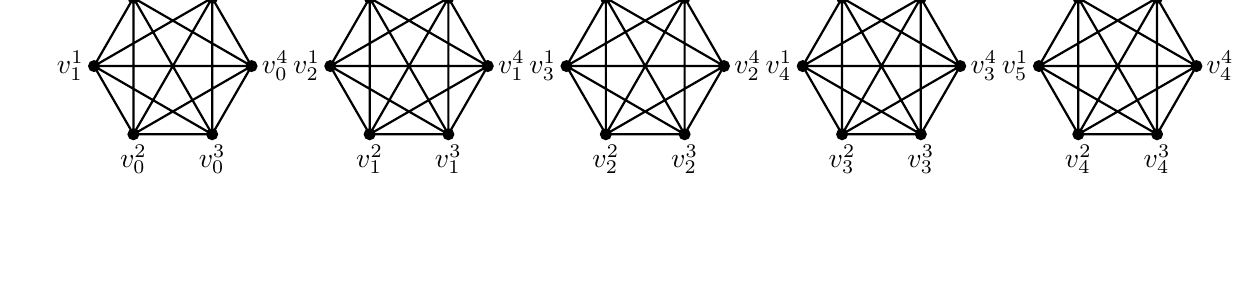
\begin{tikzpicture}[scale=1]

	\tikzstyle probe=[thick];
	\tikzstyle fragment lines=[thick];
	\tikzstyle probe lines=[thick];

	
	\filldraw[probe] (.5,1.732) circle (1.75pt) node[anchor=south] {$v^0_2$};
	\filldraw[probe] (0,.866) circle (1.75pt) node[anchor=east]{$v^1_1$};
	\filldraw[probe] (1.5,1.732) circle (1.75pt) node[anchor=south] {$v^5_0$};
	\filldraw[probe] (2,.866) circle (1.75pt) node[anchor=west]{$v^4_0$};
	\filldraw[probe] (.5,0) circle  (1.75pt) node[anchor=north]{$v^2_0$};
	\filldraw[probe] (1.5,0) circle  (1.75pt) node[anchor=north]{$v^3_0$};
	\draw[probe lines] (.5,1.732) -- (0,.866) -- (1.5,1.732) -- (2,.866) -- (.5,0) -- (1.5,1.732) -- (1.5,0) -- (.5,1.732) -- (1.5,1.732) -- (2,.866) -- (.5,1.732) -- (.5,0) -- (1.5,0) --  (2,.866) -- (.5,0) -- (.5,1.732) -- (2,.866) -- (0,.866) -- (.5,0) -- (1.5,0)--(0,.866);
	
	
		\filldraw[probe] (3.5,1.732) circle (1.75pt) node[anchor=south] {$v^0_3$};
	\filldraw[probe] (3,.866) circle (1.75pt) node[anchor=east]{$v^1_2$};
	\filldraw[probe] (4.5,1.732) circle (1.75pt) node[anchor=south] {$v^5_1$};
	\filldraw[probe] (5,.866) circle (1.75pt) node[anchor=west]{$v^4_1$};
	\filldraw[probe] (3.5,0) circle  (1.75pt) node[anchor=north]{$v^2_1$};
	\filldraw[probe] (4.5,0) circle  (1.75pt) node[anchor=north]{$v^3_1$};
	\draw[probe lines] (3.5,1.732) -- (3,.866) -- (4.5,1.732) -- (5,.866) -- (3.5,0) -- (4.5,1.732) -- (4.5,0) -- (3.5,1.732) -- (4.5,1.732) -- (5,.866) -- (3.5,1.732) -- (3.5,0) -- (4.5,0) --  (5,.866) -- (3.5,0) -- (3.5,1.732) -- (5,.866) -- (3,.866) -- (3.5,0) -- (4.5,0)--(3,.866);
	
		\filldraw[probe] (6.5,1.732) circle (1.75pt) node[anchor=south] {$v^0_4$};
	\filldraw[probe] (6,.866) circle (1.75pt) node[anchor=east]{$v^1_3$};
	\filldraw[probe] (7.5,1.732) circle (1.75pt) node[anchor=south] {$v^5_2$};
	\filldraw[probe] (8,.866) circle (1.75pt) node[anchor=west]{$v^4_2$};
	\filldraw[probe] (6.5,0) circle  (1.75pt) node[anchor=north]{$v^2_2$};
	\filldraw[probe] (7.5,0) circle  (1.75pt) node[anchor=north]{$v^3_2$};
	\draw[probe lines] (6.5,1.732) -- (6,.866) -- (7.5,1.732) -- (8,.866) -- (6.5,0) -- (7.5,1.732) -- (7.5,0) -- (6.5,1.732) -- (7.5,1.732) -- (8,.866) -- (6.5,1.732) -- (6.5,0) -- (7.5,0) --  (8,.866) -- (6.5,0) -- (6.5,1.732) -- (8,.866) -- (6,.866) -- (6.5,0) -- (7.5,0)--(6,.866);
	
		\filldraw[probe] (9.5,1.732) circle (1.75pt) node[anchor=south] {$v^0_5$};
	\filldraw[probe] (9,.866) circle (1.75pt) node[anchor=east]{$v^1_4$};
	\filldraw[probe] (10.5,1.732) circle (1.75pt) node[anchor=south] {$v^5_3$};
	\filldraw[probe] (11,.866) circle (1.75pt) node[anchor=west]{$v^4_3$};
	\filldraw[probe] (9.5,0) circle  (1.75pt) node[anchor=north]{$v^2_3$};
	\filldraw[probe] (10.5,0) circle  (1.75pt) node[anchor=north]{$v^3_3$};
	\draw[probe lines] (9.5,1.732) -- (9,.866) -- (10.5,1.732) -- (11,.866) -- (9.5,0) -- (10.5,1.732) -- (10.5,0) -- (9.5,1.732) -- (10.5,1.732) -- (11,.866) -- (9.5,1.732) -- (9.5,0) -- (10.5,0) --  (11,.866) -- (9.5,0) -- (9.5,1.732) -- (11,.866) -- (9,.866) -- (9.5,0) -- (10.5,0)--(9,.866);
	
		\filldraw[probe] (12.5,1.732) circle (1.75pt) node[anchor=south] {$v^0_6$};
	\filldraw[probe] (12,.866) circle (1.75pt) node[anchor=east]{$v^1_5$};
	\filldraw[probe] (13.5,1.732) circle (1.75pt) node[anchor=south] {$v^5_4$};
	\filldraw[probe] (14,.866) circle (1.75pt) node[anchor=west]{$v^4_4$};
	\filldraw[probe] (12.5,0) circle  (1.75pt) node[anchor=north]{$v^2_4$};
	\filldraw[probe] (13.5,0) circle  (1.75pt) node[anchor=north]{$v^3_4$};
	\draw[probe lines] (12.5,1.732) -- (12,.866) -- (13.5,1.732) -- (14,.866) -- (12.5,0) -- (13.5,1.732) -- (13.5,0) -- (12.5,1.732) -- (13.5,1.732) -- (14,.866) -- (12.5,1.732) -- (12.5,0) -- (13.5,0) --  (14,.866) -- (12.5,0) -- (12.5,1.732) -- (14,.866) -- (12,.866) -- (12.5,0) -- (13.5,0)--(12,.866);


	%\filldraw[probe] (-6,0) circle (1.75pt);
		
	

\end{tikzpicture}
\caption{Multiple Map Alignment: Graph Representation. As you can see this results in a series of clique subgraphs.}

\end{center}
\end{figure}

\paragraph{Multiple Map Alignment as the Union of Pairwise Alignments\newline}
\par{
Let us call this multiple alignment graph $G$, consisting of a set of vertices $V$ and a set of edges $E$. We can, for each pair $j$ and $l$, define $E_{jl}=E_{lj}=(u,v)$ in E such that $u.m = j$ and $v.m = l$. Since each pair of events $(u,v)$ in E comes from exactly one pair of different maps, the set of all $E_{jl}$ is a partitioning of $E$. $E_{jl}$ defines a \textbf{pairwise} alignment between maps $j$ and $l$, consisting of the pairs of homologous events between these two maps.  That {$E_{jl}$} is a partitioning of $E$ is also to say that $E$ is the union over all such pairwise alignments.  So one way to determine the perfect multiple alignment between a collection of maps is to take the union of perfect pairwise alignments.
}
\par{
But as a result of the noise described above for the Nabsys technology, a given pairwise alignment is rarely perfect.  As a result of missing and erroneous probe site measurements, however, it is not strictly intuitive what we even mean by a perfect alignment.  Consider two maps, x and y, with events $x_{1...m}$ and $y_{1...n}$.   Each event derives either from a genomic site $\gamma$ or from a false positive.  In the latter case, the event is not homologous to an event on any other map and a perfect pairwise alignment will not include this event in a matched pair.  In the former case, this event will be matched if and only if the other map has an event deriving from $\gamma$.  So the ordered set of aligned points in a perfect pairwise alignment consists of one matched pair for each event in the intersection of true positives in the two maps.
}

\begin{figure}[h!]

\begin{center}
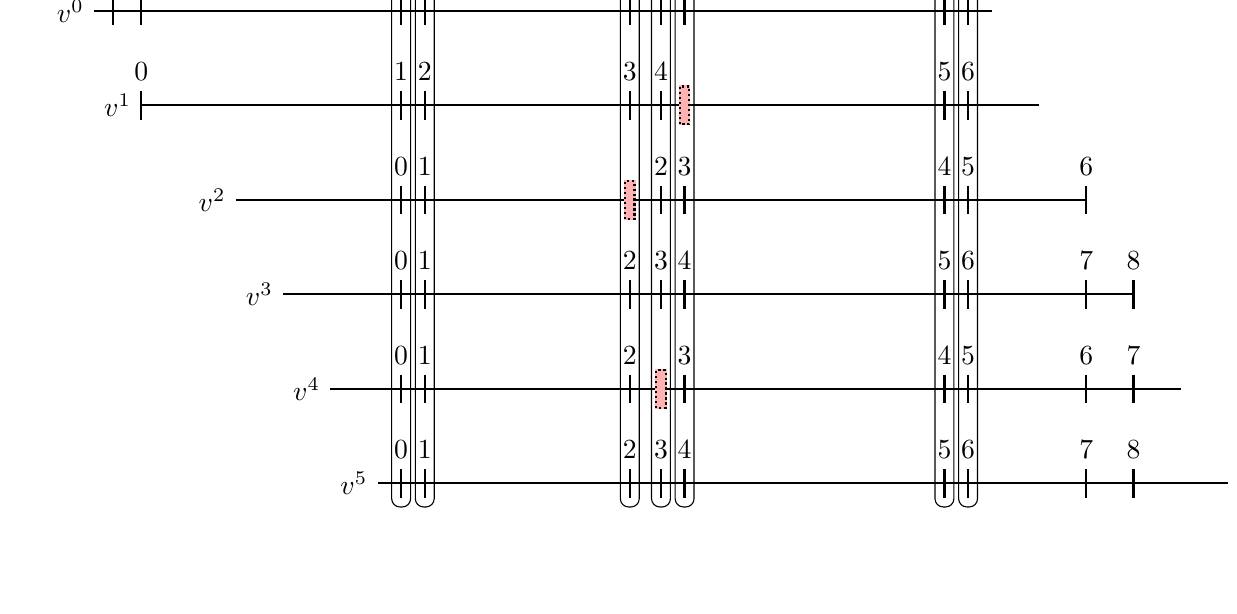
\begin{tikzpicture}[scale=1.2]

	\tikzstyle alignment lines=[densely dashed, thick];
	\tikzstyle fragment lines=[thick];
	\tikzstyle probe lines=[thick];
	\tikzstyle multiple alignment=[rounded corners=3pt];

	\draw[fragment lines] (-6,5) node[anchor=east] {$v^0$} -- (3.5,5);
		\foreach \x/\label in {-5.8/0,-5.5/1,-2.75/2,-2.5/3,-.33/4,0/5,0.25/6,3/7,3.25/8}
			\draw[probe lines,xshift=\x cm] (0,4.85) -- (0,5.15) node[anchor=south] {$\label$};

	\draw[fragment lines] (-5.5,4) node[anchor=east] {$v^1$}  -- (4,4);
		\foreach \x/\y in {-5.5/0,-2.75/1,-2.5/2,-.33/3,0/4,3/5,3.25/6}
			\draw[probe lines,xshift=\x cm] (0,4.15) node[anchor=south] {$\y$} -- (0,3.85) ;
			
			\draw[fragment lines] (-4.5,3) node[anchor=east] {$v^2$}  -- (4.5,3);
		\foreach \x/\y in {-2.75/0,-2.5/1,0/2,0.25/3,3/4,3.25/5,4.5/6}
			\draw[probe lines,xshift=\x cm] (0,3.15)node[anchor=south] {$\y$} -- (0,2.85) ;
			
					\draw[fragment lines] (-4,2) node[anchor=east] {$v^3$}  -- (5,2);
		\foreach \x/\y in {-2.75/0,-2.5/1,-.33/2,0/3,.25/4,3/5,3.25/6,4.5/7,5/8}
			\draw[probe lines,xshift=\x cm] (0,2.15) node[anchor=south] {$\y$} -- (0,1.85) ;
			
								\draw[fragment lines] (-3.5,1) node[anchor=east] {$v^4$}  -- (5.5,1);
		\foreach \x/\y in {-2.75/0,-2.5/1,-.33/2,.25/3,3/4,3.25/5,4.5/6,5/7}
			\draw[probe lines,xshift=\x cm] (0,1.15) node[anchor=south] {$\y$} -- (0,.85) ;
			
								\draw[fragment lines] (-3,0) node[anchor=east] {$v^5$}  -- (6,0);
		\foreach \x/\y in {-2.75/0,-2.5/1,-.33/2,0/3,.25/4,3/5,3.25/6,4.5/7,5/8}
			\draw[probe lines,xshift=\x cm] (0,.15) node[anchor=south] {$\y$} -- (0,-.15) ;
		
		%\foreach \x in {-2.75,-2.5,0,2,3}
		%	\draw[alignment lines, xshift=\x cm] (0,.18) -- (0,.82);
		
		\draw[multiple alignment] (-2.85,-.25) rectangle (-2.65,5.65);
		\draw[multiple alignment] (-2.6,-.25) rectangle (-2.4,5.65);
		\draw[multiple alignment] (-.1,-.25) rectangle (.1,5.65);
		\draw[multiple alignment] (3.15,-.25) rectangle (3.35,5.65);
		\draw[multiple alignment] (2.9,-.25) rectangle (3.1,5.65);
		\draw[multiple alignment] (-.43,-.25) rectangle (-.23,5.65);
		\draw[multiple alignment] (.15,-.25) rectangle (.35,5.65);
		
		\filldraw[red!30, thick] (.2,3.8) rectangle (.3,4.2);
		\draw[thick, densely dotted] (.2,3.8) rectangle (.3,4.2);
		
		\filldraw[red!30, thick] (-.38,2.8) rectangle (-.28,3.2);
		\draw[thick, densely dotted] (-.38,2.8) rectangle (-.28,3.2);
		
		\filldraw[red!30, thick] (-.05,.8) rectangle (.05,1.2);
		\draw[thick, densely dotted] (-.05,.8) rectangle (.05,1.2);
		
		
		%\draw (-2.75,2.75) ellipse (5pt and 3cm);
		%\draw (-2.5,2.75) ellipse (5pt and 3cm);
		%\draw (0,2.75) ellipse (5pt and 3cm);
		%\draw (2,2.75) ellipse (5pt and 3cm);
		%\draw (3,2.75) ellipse (5pt and 3cm);

\end{tikzpicture}
 \caption{Multiple Map Alignment: An example.  Here we see that several of our maps have false negatives in them.  The circled probes are the desired multiple alignment but it will turn out that not all of the pairwise alignments agree with this.}
\end{center}
\end{figure}

\begin{figure}[h!]
\begin{center}
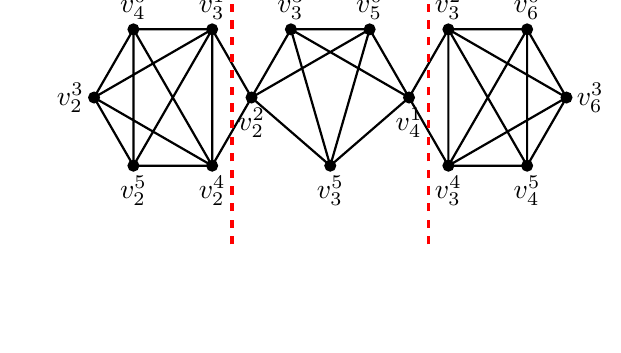
\begin{tikzpicture}[scale=1]

	\tikzstyle probe=[thick];
	\tikzstyle fragment lines=[thick];
	\tikzstyle probe lines=[thick];

	
	\filldraw[probe] (.5,1.732) circle (1.75pt) node[anchor=south] {$v^0_4$};
	\filldraw[probe] (0,.866) circle (1.75pt) node[anchor=east]{$v^3_2$};
	\filldraw[probe] (1.5,1.732) circle (1.75pt) node[anchor=south] {$v^1_3$};
	\filldraw[probe] (2,.866) circle (1.75pt) node[anchor=north]{$v^2_2$};
	\filldraw[probe] (.5,0) circle  (1.75pt) node[anchor=north]{$v^5_2$};
	\filldraw[probe] (1.5,0) circle  (1.75pt) node[anchor=north]{$v^4_2$};
	\draw[probe lines] (.5,1.732) -- (0,.866) -- (1.5,1.732)  -- (1.5,1.732) -- (1.5,0) -- (.5,1.732) -- (1.5,1.732) -- (.5,1.732) -- (.5,0) --(0,.866) --(1.5,0) --(.5,0) --(1.5,1.732) -- (1.5,0) -- (2,.866);
	%\draw[probe lines] 
	%\draw[probe lines] 
	%\draw[probe lines] 
	%\draw[probe lines] 
	%\draw[probe lines] 
	
	%(.5,1.732) -- (0,.866) -- (1.5,1.732) -- (2,.866) -- (.5,0) -- (1.5,1.732) -- (1.5,0) -- (.5,1.732) -- (1.5,1.732) -- (2,.866) -- (.5,1.732) -- (.5,0) -- (1.5,0) --  (2,.866) -- (.5,0) -- (.5,1.732) -- (2,.866) -- (1.5,0)--(0,.866) -- (.5,0);
	
	
		\filldraw[probe] (2.5,1.732) circle (1.75pt) node[anchor=south] {$v^3_3$};
	%\filldraw[probe] (3,.866) circle (1.75pt) node[anchor=east]{$v^1_2$};
	\filldraw[probe] (3.5,1.732) circle (1.75pt) node[anchor=south] {$v^0_5$};
	%\filldraw[probe] (5,.866) circle (1.75pt) node[anchor=west]{$v^4_1$};
	\filldraw[probe] (3,0) circle  (1.75pt) node[anchor=north]{$v^5_3$};
	%\filldraw[probe] (4.5,0) circle  (1.75pt) node[anchor=north]{$v^3_1$};
	\draw[probe lines] (1.5,1.732) -- (2,.866) -- (3.5,1.732) -- (4,.866) -- (3,0) -- (3.5,1.732) -- (3,0) -- (2.5,1.732) -- (3.5,1.732) -- (4,.866) -- (2.5,1.732) -- (3,0) --  (4,.866) -- (3,0) -- (2.5,1.732)  -- (2,.866) -- (3,0);
	
		\filldraw[probe] (4.5,1.732) circle (1.75pt) node[anchor=south] {$v^2_3$};
	\filldraw[probe] (4,.866) circle (1.75pt) node[anchor=north]{$v^1_4$};
	\filldraw[probe] (5.5,1.732) circle (1.75pt) node[anchor=south] {$v^0_6$};
	\filldraw[probe] (6,.866) circle (1.75pt) node[anchor=west]{$v^3_6$};
	\filldraw[probe] (4.5,0) circle  (1.75pt) node[anchor=north]{$v^4_3$};
	\filldraw[probe] (5.5,0) circle  (1.75pt) node[anchor=north]{$v^5_4$};
	\draw[probe lines] (4.5,1.732)  -- (5.5,1.732) -- (6,.866) -- (4.5,0) -- (5.5,1.732) -- (5.5,0) -- (4.5,1.732) -- (5.5,1.732) -- (6,.866) -- (4.5,1.732) -- (4.5,0) -- (5.5,0) --  (6,.866) -- (4.5,0) -- (4.5,1.732) -- (6,.866)  -- (4.5,0) -- (5.5,0) -- (4.5,0) -- (4,.866) -- (4.5,1.732);
	
	
	\draw[red,dashed, very thick] (4.25,-1) -- (4.25,2.732);
	
	\draw[red,dashed, very thick] (1.75,-1) -- (1.75,2.732);
	
	%\filldraw[probe] (-6,0) circle (1.75pt);
		
	

\end{tikzpicture}
\caption{Multiple Map Alignment: Graph Representation. This example refers to the alignments of the maps contained in figure 7.  This alignment graph contains multiple \textbf{contradictions}.  Note that the vertices have been rearranged spatially for ease of viewing the graph.  The broken red lines indicate the edges that must be cut in order to obtain the contradiction-free multiple alignment that best explains all of the pairwise alignments.}
\end{center}
\end{figure}


\paragraph{Modified-Karger's Algorithm for Contradiction Separation\newline}
\par{
Suppose that we have performed pairwise alignments between all pairs of input maps.  Consider the set of edges $E^\prime$ (and the graph $G^\prime={V,E^\prime}$) formed by taking the union of these imperfect pairwise alignments.  $E^\prime$ differs from the perfect solution $E$ in its missing and extra edges.  Most importantly, the extra edges mean that $E^\prime$ has edges between what would be separated components in $E$.  (Additionally, some edges are missing within what would be connected components in $E$. These missing edges are less of a concern under the assumed coverage because it is very unlikely that enough edges might be missing to separate a connected component into two or more components.) In order to recover $E$ as best possible, we set about removing the extra edges from $E^\prime$.
}
\par{
The extra edges in $E^\prime$ have the property that they introduce \textbf{contradictions}.  Let us define a contradiction as a connected component in $G^\prime$ that contains two or more different vertices from the same map.  This means that the multiple alignment implicit from $G^\prime$ currently counts two events on one measurement map as arising from a single event in the underlying true map.  This is always an error because each aligned point in our multiple alignment should correspond to a particular event $\gamma$ in the map of common origin and it is impossible for two sites on the same map to be homologous to the same $\gamma$.  One important step towards fixing $E^\prime$ is to separate these \textbf{contradictory components} into non-contradictory ones.
}

\begin{figure}[h!]
\begin{center}
\begin{tikzpicture}[scale=1]

	\tikzstyle alignment lines=[densely dashed, thick];
	\tikzstyle fragment lines=[thick];
	\tikzstyle probe lines=[thick];

	\draw[fragment lines] (-6,1) node[anchor=east] {$v^0$} -- (-1,1);
		\foreach \x/\label in {-3.2/0,-2.8/1}
			\draw[probe lines,xshift=\x cm] (0,.85) -- (0,1.15) node[anchor=south] {$\label$};

	\draw[fragment lines] (-5,0) node[anchor=east] {$v^1$}  -- (0,0);
		\foreach \x/\y in {-3/0}
			\draw[probe lines,xshift=\x cm] (0,.15) -- (0,-.15) node[anchor=north] {$\y$};
			
	\draw[fragment lines] (1,1) node[anchor=east] {$v^0$}  -- (6,1);
		\foreach \x/\y in {3.8/0,4.2/1}
			\draw[probe lines,xshift=\x cm] (0,.85) -- (0,1.15) node[anchor=south] {$\y$};
	\draw[fragment lines] (3,0) node[anchor=east] {$v^2$}  -- (8,0);
		\foreach \x/\y in {4/0}
			\draw[probe lines,xshift=\x cm] (0,.15) -- (0,-.15) node[anchor=north] {$\y$};
			
	\draw[fragment lines] (-2,-1) node[anchor=east] {$v^1$}  -- (3,-1);
		\foreach \x/\y in {0/0}
			\draw[probe lines,xshift=\x cm] (0,-.85) node[anchor=south]  {$\y$} -- (0,-1.15) ;
	\draw[fragment lines] (-1,-2) node[anchor=east] {$v^2$}  -- (4,-2);
		\foreach \x/\y in {0/0}
			\draw[probe lines,xshift=\x cm] (0,-1.85) -- (0,-2.15) node[anchor=north] {$\y$};
		
		\draw[alignment lines] (-3,.18)--(-3.2,.82);
		
		\draw[alignment lines] (4.2,.82)--(4,.18);
		
		\draw[alignment lines] (0,-1.82)--(0,-1.18);
		%\foreach \x in {-2.75,-2.5,0,2,3}
		%	\draw[alignment lines, xshift=\x cm] (0,.18) -- (0,.82);

\end{tikzpicture}
\caption{  An example of a contradictory set of pairwise alignments.  Here $v^0_0$ is aligned to $v^1_0$ which is aligned to $v^2_0$ but in the alignment between maps $0$ and $2$ $v^0_1$ is aligned to $v^2_0$. These are inconsistent assignments of homology and therefore a contradiction.}
\end{center}
\end{figure}




\par{
Under the presumption that most edges in $E^\prime$ are correct, a natural way to fix these contradictions is to find a min-cut such that no contradictions remain.  We use a novel, modified version of Karger's Algorithm to find this min-cut.  Karger's Algorithm is a probabilistic algorithm that finds the min-cut of a graph by finding strongly connected components and then severing them from one another.  These strongly connected components are discovered by "contracting" edges at random until only two nodes remain.  To contract an edge is to remove the edge and combine its end nodes into one node retaining all other edges therefore allowing multiple edges between two nodes.  The selected cut itself is the set of all edges remaining when no further contraction is allowed.  This process can of course fail to find the min-cut.  Consider for instance that the first edge contracted at random happens to be an edge that is in the min cut.  For this reason we must perform this succession of contractions many times in parallel and selecting the minimum cut among these iterations, the algorithm offers high probability of finding the min-cut.  Because strongly connected components contain far more edges than other areas of the graph, these areas get contracted earlier with higher probability.  This convenient property of highly connected components allows for very high probability of finding the real min-cut with surprisingly few iterations.  This run time can be further improved by a modification known as the Karger-Stein algorithm.  In our case, we impose the additional constraint that no two vertices representing events on the same map can be contracted.  This constraint is natural because the fully-contracted vertices at the end of Karger's Algorithm are identical to the \textbf{aligned points} our multiple alignment seeks to recover.  As such, our modified Karger's Algorithm contracts edges at random without violating constraints until no contractions are allowed under the constraints.  The min-cut selected by this modified Karger's Algorithm represents a likely selection of the extra edges in $E^\prime$ and, in any case, results in an ordered set of non-contradictory connected components that best explain the set of pairwise alignments.\cite{Karger1}\cite{Karger2}
 As a simplified example, take the following set of fragments.}


\begin{figure}[h!]

\begin{center}
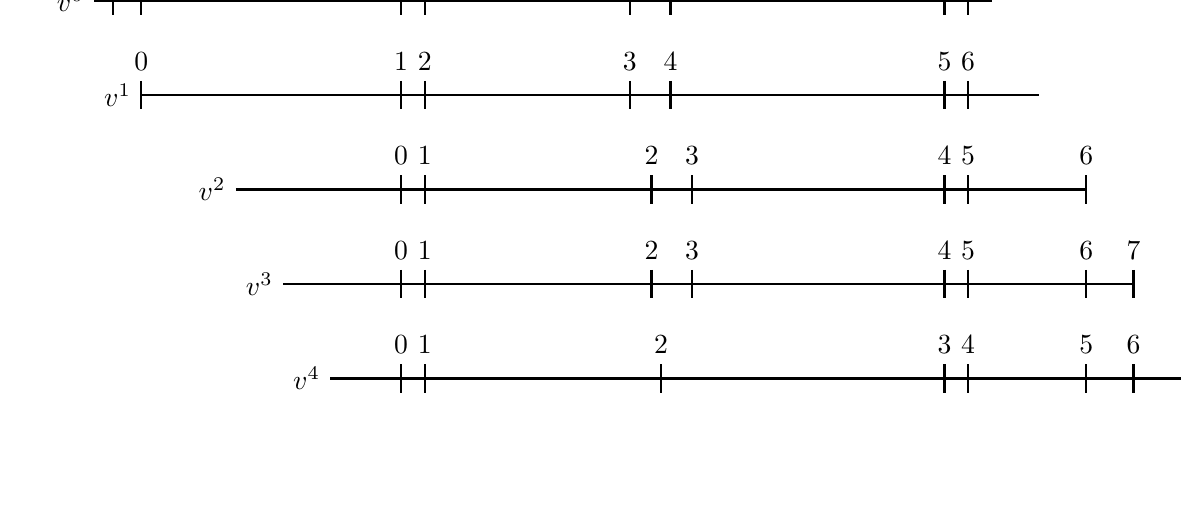
\begin{tikzpicture}[scale=1.2]

	\tikzstyle alignment lines=[densely dashed, thick];
	\tikzstyle fragment lines=[thick];
	\tikzstyle probe lines=[thick];
	\tikzstyle multiple alignment=[rounded corners=3pt];

	\draw[fragment lines] (-6,5) node[anchor=east] {$v^0$} -- (3.5,5);
		\foreach \x/\label in {-5.8/0,-5.5/1,-2.75/2,-2.5/3,-.33/4,0.1/5,3/6,3.25/7}
			\draw[probe lines,xshift=\x cm] (0,4.85) -- (0,5.15) node[anchor=south] {$\label$};
			
	

	\draw[fragment lines] (-5.5,4) node[anchor=east] {$v^1$}  -- (4,4);
		\foreach \x/\y in {-5.5/0,-2.75/1,-2.5/2,-.33/3,0.1/4,3/5,3.25/6}
			\draw[probe lines,xshift=\x cm] (0,4.15) node[anchor=south] {$\y$} -- (0,3.85) ;
			
	\draw[fragment lines] (-4.5,3) node[anchor=east] {$v^2$}  -- (4.5,3);
		\foreach \x/\y in {-2.75/0,-2.5/1,-.1/2,0.33/3,3/4,3.25/5,4.5/6}
			\draw[probe lines,xshift=\x cm] (0,3.15)node[anchor=south] {$\y$} -- (0,2.85) ;
			
					\draw[fragment lines] (-4,2) node[anchor=east] {$v^3$}  -- (5,2);
		\foreach \x/\y in {-2.75/0,-2.5/1,-.1/2,.33/3,3/4,3.25/5,4.5/6,5/7}
			\draw[probe lines,xshift=\x cm] (0,2.15) node[anchor=south] {$\y$} -- (0,1.85) ;
			
								\draw[fragment lines] (-3.5,1) node[anchor=east] {$v^4$}  -- (5.5,1);
		\foreach \x/\y in {-2.75/0,-2.5/1,0/2,3/3,3.25/4,4.5/5,5/6}
			\draw[probe lines,xshift=\x cm] (0,1.15) node[anchor=south] {$\y$} -- (0,.85) ;
			
								%\draw[fragment lines] (-3,0) node[anchor=east] {$v^5$}  -- (6,0);
		%\foreach \x/\y in {-2.75/0,-2.5/1,-.33/2,0/3,.25/4,3/5,3.25/6,4.5/7,5/8}
		%	\draw[probe lines, xshift=\x cm] (0,.15) node[anchor=south] {$\y$} -- (0,-.15) ;
		
		%\foreach \x in {-2.75,-2.5,0,2,3}
		%	\draw[alignment lines, xshift=\x cm] (0,.18) -- (0,.82);
		
		%\draw[multiple alignment] (-2.85,-.25) rectangle (-2.65,5.65);
		%\draw[multiple alignment] (-2.6,-.25) rectangle (-2.4,5.65);
		%\draw[multiple alignment] (-.1,-.25) rectangle (.1,5.65);
		%\draw[multiple alignment] (3.15,-.25) rectangle (3.35,5.65);
		%\draw[multiple alignment] (2.9,-.25) rectangle (3.1,5.65);
		%\draw[multiple alignment] (-.43,-.25) rectangle (-.23,5.65);
		%\draw[multiple alignment] (.15,-.25) rectangle (.35,5.65);
		
		%\filldraw[red!30, thick] (.2,3.8) rectangle (.3,4.2);
		%\draw[thick, densely dotted] (.2,3.8) rectangle (.3,4.2);
		
		%\filldraw[red!30, thick] (-.38,2.8) rectangle (-.28,3.2);
		%\draw[thick, densely dotted] (-.38,2.8) rectangle (-.28,3.2);
		
		%\filldraw[red!30, thick] (-.05,.8) rectangle (.05,1.2);
		%\draw[thick, densely dotted] (-.05,.8) rectangle (.05,1.2);
		
		
		%\draw (-2.75,2.75) ellipse (5pt and 3cm);
		%\draw (-2.5,2.75) ellipse (5pt and 3cm);
		%\draw (0,2.75) ellipse (5pt and 3cm);
		%\draw (2,2.75) ellipse (5pt and 3cm);
		%\draw (3,2.75) ellipse (5pt and 3cm);

\end{tikzpicture}
 \caption{An example set of fragments on which one iteration of our modified Karger's algorithm will be demonstrated in figure 11. Note how the pairwise alignments for these fragments will be in contradiction due to fragment 4 probe 2.}
\end{center}
\end{figure}
\begin{figure}[h!]
\begin{center}
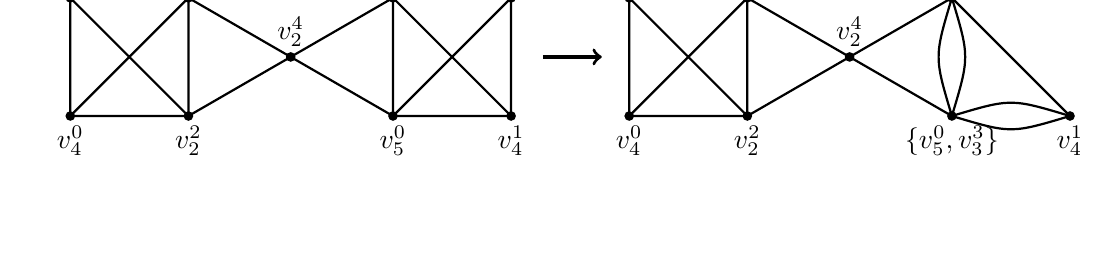
\begin{tikzpicture}[scale=.75]

	\tikzstyle probe=[thick];
	\tikzstyle fragment lines=[thick];
	\tikzstyle probe lines=[thick];

	
	\filldraw[probe] (0,0) circle (1.75pt) node[anchor=north] {$v^0_4$};
	\filldraw[probe] (0,2) circle (1.75pt) node[anchor=south]{$v^1_3$};
	\filldraw[probe] (2,0) circle (1.75pt) node[anchor=north] {$v^2_2$};
	\filldraw[probe] (2,2) circle (1.75pt) node[anchor=south]{$v^3_2$};
	%\filldraw[probe] (.5,0) circle  (1.75pt) node[anchor=north]{$v^5_2$};
	%\filldraw[probe] (1.5,0) circle  (1.75pt) node[anchor=north]{$v^4_2$};
	\draw[probe lines] (0,0) -- (0,2) -- (2,0) -- (2,2) -- (0,2) -- (2,0) -- (0,0) -- (2,2);
	%\draw[probe lines] 
	%\draw[probe lines] 
	%\draw[probe lines] 
	%\draw[probe lines] 
	%\draw[probe lines] 
	
	%(.5,1.732) -- (0,.866) -- (1.5,1.732) -- (2,.866) -- (.5,0) -- (1.5,1.732) -- (1.5,0) -- (.5,1.732) -- (1.5,1.732) -- (2,.866) -- (.5,1.732) -- (.5,0) -- (1.5,0) --  (2,.866) -- (.5,0) -- (.5,1.732) -- (2,.866) -- (1.5,0)--(0,.866) -- (.5,0);
	
	
		%\filldraw[probe] (2.5,1.732) circle (1.75pt) node[anchor=south] {$v^3_3$};
	%\filldraw[probe] (3,.866) circle (1.75pt) node[anchor=east]{$v^1_2$};
	\filldraw[probe] (3.732,1) circle (1.75pt) node[anchor=south] {$v^4_2$};
	%\filldraw[probe] (5,.866) circle (1.75pt) node[anchor=west]{$v^4_1$};
	%\filldraw[probe] (3,0) circle  (1.75pt) node[anchor=north]{$v^5_3$};
	%\filldraw[probe] (4.5,0) circle  (1.75pt) node[anchor=north]{$v^3_1$};
	\draw[probe lines] (3.732,1) -- (5.464,0);
	\draw[probe lines] (3.732,1) -- (5.464,2);
	\draw[probe lines] (3.732,1) -- (2,0);
	\draw[probe lines] (3.732,1) -- (2,2);
	
	\filldraw[probe] (5.464,0) circle (1.75pt) node[anchor=north] {$v^0_5$};
	\filldraw[probe] (7.464,0) circle (1.75pt) node[anchor=north]{$v^1_4$};
	\filldraw[probe] (5.464,2) circle (1.75pt) node[anchor=south] {$v^2_3$};
	\filldraw[probe] (7.464,2) circle (1.75pt) node[anchor=south]{$v^3_3$};
%	\filldraw[probe] (4.5,0) circle  (1.75pt) node[anchor=north]{$v^4_3$};
	%\filldraw[probe] (5.5,0) circle  (1.75pt) node[anchor=north]{$v^5_4$};
	\draw[probe lines] (5.464,0) -- (5.464,2) -- (7.464, 2) -- (5.464,2) -- (7.464,0) -- (5.464,0) -- (7.464,2) -- (7.464,0);
	
	\draw[very thick,->] (8,1) -- (9,1);
	
	\filldraw[probe] (9.464,0) circle (1.75pt) node[anchor=north] {$v^0_4$};
	\filldraw[probe] (9.464,2) circle (1.75pt) node[anchor=south]{$v^1_3$};
	\filldraw[probe] (11.464,0) circle (1.75pt) node[anchor=north] {$v^2_2$};
	\filldraw[probe] (11.464,2) circle (1.75pt) node[anchor=south]{$v^3_2$};
	%\filldraw[probe] (.5,0) circle  (1.75pt) node[anchor=north]{$v^5_2$};
	%\filldraw[probe] (1.5,0) circle  (1.75pt) node[anchor=north]{$v^4_2$};
	\draw[probe lines] (9.464,0) -- (9.464,2) -- (11.464,0) -- (11.464,2) -- (9.464,2) -- (11.464,0) -- (9.464,0) -- (11.464,2);
	
		\filldraw[probe] (13.196,1) circle (1.75pt) node[anchor=south] {$v^4_2$};
	%\filldraw[probe] (5,.866) circle (1.75pt) node[anchor=west]{$v^4_1$};
	%\filldraw[probe] (3,0) circle  (1.75pt) node[anchor=north]{$v^5_3$};
	%\filldraw[probe] (4.5,0) circle  (1.75pt) node[anchor=north]{$v^3_1$};
	\draw[probe lines] (13.196,1) -- (11.464,0);
	\draw[probe lines] (13.196,1) -- (11.464,2);
	\draw[probe lines] (13.196,1) -- (14.928,0);
	\draw[probe lines] (13.196,1) -- (14.928,2);
	
		\filldraw[probe] (14.928,0) circle (1.75pt) node[anchor=north] {$\{v^0_5,v^3_3\}$};
	\filldraw[probe] (16.928,0) circle (1.75pt) node[anchor=north]{$v^1_4$};
	\filldraw[probe] (14.928,2) circle (1.75pt) node[anchor=south] {$v^2_3$};
%	\filldraw[probe] (4.5,0) circle  (1.75pt) node[anchor=north]{$v^4_3$};
	%\filldraw[probe] (5.5,0) circle  (1.75pt) node[anchor=north]{$v^5_4$};
	\draw[probe lines]  (14.928,2) -- (16.928,0);
	\draw[probe lines] (14.928,0) ..  controls (15.228,1) .. (14.928,2);
	\draw[probe lines] (14.928,0) ..  controls (14.628,1) .. (14.928,2);
	
	\draw[probe lines] (14.928,0) ..  controls (15.928,.3)  .. (16.928,0);
	\draw[probe lines] (14.928,0) ..  controls (15.928,-.3) .. (16.928,0);


	
	
	%\draw[red,dashed, very thick] (4.25,-1) -- (4.25,2.732);
	
	%\draw[red,dashed, very thick] (1.75,-1) -- (1.75,2.732);
	
	%\filldraw[probe] (-6,0) circle (1.75pt);
		
	

\end{tikzpicture}
\caption{Contraction on edge from $v^0_5$ to $v^3_3$. Edges are drawn at random and contracted if they do not have labels of the same fragment (the superscript here). This process continues until either there are 2 nodes left in the graph and the remaining edges are the ``cut" or no more edges can be contracted given our constraint. This process is then repeated several times and the cut with the fewest cut edges is selected as the most likely.}

\end{center}
\end{figure}


\par{
Karger's Algorithm, along with our modifications, is uniquely suited to this problem.  No other formulation of the min-cut problem (network flow, etc.) can be so simply extended with our constraints.  The operation of Karger's Algorithm consists of a probabilistic sampling of the space of graph cuts.  By introducing our constraints, we simple decline to sample the portion of the space that contains contradictions.  And, if this was not clear, in the simple case in which $E^\prime$ contains no contradictions to begin with we do nothing and just take it as the multiple alignment.  
}



\paragraph{De Novo Genetic Map Assembly: The Problem and Complexity\newline}
\par{
De novo genetic map assembly is a problem several other groups have tackled\cite{Opgen2}\cite{Opgen3}\cite{OpgenHaplotype}\cite{ValouevRefinement}\cite{ValouevAssembler} but due to time complexity none of these easily extends to large mammalian genomes.  The exceptions to this are Opgen's human mapping with help from a reference\cite{OpgenHuman} and Maize mapping with a cluster of servers using an iterative divide and conquer method\cite{OpgenMaize} as well as Opgen's rice genome mapping done in the same manner.  The reason for these difficulties is that the algorithms that are the building blocks of assembly (pairwise alignment and multiple alignment) have inherently higher complexity than their sequencing counterparts.  The well defined algorithm of pairwise alignment has $O(n^2)$ complexity for sequence alignment where $n$ is the number of bases.  In contrast, map alignment has complexity $O(n^4)$ where $n$ is the number of events. Furthermore, because sequencing error rates are initially an averaging over many molecules, the resulting reads have relatively little error.  This allows assemblers to look at exact matches of certain lengths of sequences. Hashing reads by these exact values allows for constant time lookups getting around the problem of aligning entirely. In fact, all modern sequence assemblers all are based on this concept and many employ little to no alignment.  This is, for the most part, not possible with mapping as each ``read" is a single molecule measurement which is inherently relatively noise prone. We will describe our method to utilize ``exact matches" in the section titled Fragment Selection. We include this for completion but, while unpublished, we do not believe this method to be novel.}

{The size of a genetic map assembly problem is somewhat difficult to define.  It is not simply based on the size of the genome but also the frequency with which the sequence specific target appears in that genome.  Because this frequency can vary significantly, the number of events is a much better proxy for the size of the problem than genome length is.  In a random genetic sequence of sufficient length all sequences of a particular length $K$ occur with equal probability.  In a random sequence, a given $K$-mer occurs as a poisson process with frequency $\lambda = \frac{1}{4^K}$ and the intervals between these occurrences follow a geometric distribution with $\mu=4^K$. In non-random DNA such as real genomes the frequency of a given $K$-mer may significantly different from the random model but still closely follows a poisson distribution with that particular frequency.  The size of the genetic map assembly problem grows at least linearly with the sequence specific target frequency.  The optical mapping technology targets sequences that occur at a frequency of once every 10,000 bases ($\lambda = \frac{1}{10,000}$) or more.  The Nabsys positional sequencing technology attempts to gain greater resolution by targeting sequences that occur once every 2,000-6,000 bases ($\lambda = \frac{1}{2,000}$ to $\frac{1}{6,000}$) thus creating a 2-5 fold larger computational problem.  Error level including positional, false negatives, and positives increase computational complexity in poorly defined ways.  The reason for this is that certain approximation optimizations in searching for fragments as well as in pairwise alignment are sensitive to these errors \cite{ValouevAlignment}.  We describe a method for genetic map assembly that, under our error levels, can assemble a mammalian sized genome with event frequency of one in 2,000 at 30 fold coverage in approximately one hour on a single core of a commodity sandy bridge i7 processor with $\leq 8Gb$ of ram. }



\paragraph{Fragment Selection: Signatures - A Discretized Geometric Hashing\newline}
\par{
In order to speed up the assembly process we wish to be able to efficiently search for fragments that contain a short segment that is similar to a part of the growing consensus map.  This is similar to the short sequence hashing employed in the commonly used BLAST algorithm. We define a \textbf{signature} as a ordered sequence of discretized interval lengths between $S$ events. We wish these ``signatures" to be reliable by which we mean that we wish them to be discretized to the same value as they would with no error. But we also wish to be able to search for them with constant time look up.  So we must average intervals to certain chosen discrete values.  The discretization of these intervals is designed to efficiently hash fragments into collections of roughly equal size.  To do this we make the approximation that if we chose boundaries to our discrete values such that an equal number of intervals over the entire data set fall in each then the distribution of number of ordered discretized intervals will also be uniform.  Under our simulations with reference genomes this approximation is close to accurate.  This method has performed better (created more uniformly sized signature collections) in simulation than choosing discretization boundaries purely on a geometric size basis which Opgen employs (unpublished). It is worth noting that a false positive or false negative will almost invariably make a signature incorrect while it is much less likely for positional error to do so.  There is a problem with interval sizes near the boundaries of the range encompassed by a discrete value.  These internals have a much higher probability of being made incorrect by positional error than do intervals whose lengths fall in the center of the range for a particular discrete value. }


\paragraph{Nabsys Assembly\newline}
\par{Assume we have a putative consensus map going back at least $S$ events where $S$ is a parameter usually in the range 4-6.  Make a further assumption that there is a collection of fragments that overlap the putative consensus.  We term this collection of fragments the \textbf{bundle}.  Our assembly proceeds as follows. We seed the process with a random fragment. Then at each step in the algorithm one of two events occurs.
\begin{itemize}
\item  If the bundle size is less than some number $B$ (usually 6-12), search for fragments to add to the bundle until it is of size $B$. When searching for fragments to add to the bundle, we pick a signature, attempt to align each fragment with that signature to the growing consensus.  If an alignment score passes a statistical significance test then we align the new fragment to each of the $B$ fragments that currently overlap the growing consensus.  If each of these alignment scores passes significance tests we add that fragment to the bundle.
\item If the bundle is of sufficient size then do a multiple alignment on these fragments as previously described to pick consensus events and their locations and add them to the growing consensus.
\end{itemize} When a fragment in the bundle no longer has any forward overhang it is discarded from the bundle. This process continues until we cannot find enough fragments to fill the bundle that pass these significance tests. We run this process in both direction for each contig. When one contig ends we start a new contig in the same manner as before until no further progress can be made. Sequence assemblers are built in such a way that they expose the repetitious sequences and the ambiguous nature of the assembly at those places. They do this with either an overlap graph or a DeBrujin Graph. Since our assembly proceeds in a greedy manner we do not do this.  This could potentially lead to putting together two areas that are not contiguous in the actual genome if a very long repeat occurred there. This type of error is referred to as a miss assembly or a chimeric assembly.  Repetitions of this length are not expected since we require length of the overlap of a new fragment with the growing consensus to be greater than known exact or approximate repeat structures in known genomes (15kb is sufficient for most prokaryotic genomes while 45kb is necessary for mammalian and plant genomes). But we do not rely on this fact alone. We also identify possible repetitions and ambiguities either before or after the assembly and cut contigs at these positions.\cite{assemblyReview}\cite{StringGraph}\cite{ValouevAssembler}
}
\paragraph{Conclusions\newline}

\par{
We have outlined a set of methods for de novo assembly of distance maps accurately and efficiently even under a high level of error in the input data.
}

%\paragraph{Combination Sequencing\newline}
%\par{
%Here I will talk about combination sequencing\cite{Antoniotti}\cite{Zhousingle-molecule}
%}


\bibliographystyle{amsplain}
\bibliography{patent2}
\end{document}